\documentclass{book}
\usepackage{xcolor}
\usepackage{fontspec}
\usepackage{setspace}

\usepackage{xeCJK}
\setsansfont[SlantedFont=* ]{Noto Serif CJK SC}
\setmainfont[SlantedFont=* ]{Noto Serif CJK SC}
\setCJKmainfont[SlantedFont=* ]{Noto Serif CJK SC}
\setCJKsansfont[SlantedFont=* ]{Noto Sans CJK SC}
% \setCJKmonofont{Noto Sans Mono CJK SC}

\usepackage{afterpage}

\newcommand\blankpage{%
    \null
    \thispagestyle{empty}%
    \addtocounter{page}{-1}%
    \newpage}

    \newcommand\spreadsize[3]{\linespread{#1}\fontsize{#2}{#3}\selectfont
This paragraph uses linespread=#1:
Some text to try out the result of linespread. A little more to have a least three lines on this measure. 
Finish off with a paragraph end so that linebreaking happens.\par\bigskip}
%
%	landscape orientation 
%
\usepackage[landscape]{geometry}
\usepackage{multicol}
\usepackage{graphicx}
\usepackage{geometry}
\usepackage{lipsum}
\usepackage{verbatim}
\usepackage{eso-pic}
\usepackage{fancyhdr}
\usepackage{tikz}
\usepackage{bidicontour}
\usepackage{bidi}






\begin{document}


\pagenumbering{gobble}

%****************************************
%*										*
%*										*
%****************************************
%HERE IS A GOOD COLLAGE OF PHOTOS, IT´S GOOD WITH PORTRAITS 
\begin{comment}

%BEGIN OF COLLAGE 
%BEGIN OF COLLAGE 
%BEGIN OF COLLAGE 
%BEGIN OF COLLAGE 
%BEGIN OF COLLAGE 

\newgeometry{margin=0cm}
\setlength{\parindent}{0pt}

\setlength{\tabcolsep}{0pt} 
\renewcommand{\arraystretch}{0}

\begin{tabular}{ l l l  }


\includegraphics[width=9.3cm,height=5.4cm]{./res/dummy.jpg} &

\includegraphics[width=9.3cm,height=5.4cm]{./res/dummy.jpg} & 

\includegraphics[width=9.4cm,height=5.4cm]{./res/dummy.jpg} \\


\includegraphics[width=9.3cm,height=5.4cm]{./res/dummy.jpg} &

\includegraphics[width=9.3cm,height=5.4cm]{./res/dummy.jpg} & 

\includegraphics[width=9.4cm,height=5.4cm]{./res/dummy.jpg} \\


\includegraphics[width=9.3cm,height=5.4cm]{./res/dummy.jpg} &

\includegraphics[width=9.3cm,height=5.4cm]{./res/dummy.jpg} & 

\includegraphics[width=9.4cm,height=5.4cm]{./res/dummy.jpg} \\


\includegraphics[width=9.3cm,height=5.4cm]{./res/dummy.jpg} &

\includegraphics[width=9.3cm,height=5.4cm]{./res/dummy.jpg} & 

\includegraphics[width=9.4cm,height=5.4cm]{./res/dummy.jpg} \\

\end{tabular}

\restoregeometry


%END OF COLLAGE 
%END OF COLLAGE 
%END OF COLLAGE 
%END OF COLLAGE 
\end{comment}

\bidicontourlength{0.8pt}
\bidicontour{white}{\sffamily\fontsize{11}{1}\selectfont Legends of the animals}\par
\bidicontour{white}{\sffamily\fontsize{11}{1}\selectfont 动物拍案惊奇系列}\par

\begingroup
\thispagestyle{empty}
\AddToShipoutPicture*{\put(-20,-20){
\includegraphics[scale=1.1]{./res/cover.png}}} % Image background
\centering
\vspace*{5cm}
\endgroup

\bidicontourlength{1.5pt}
\bidicontour{white}{\sffamily\fontsize{35}{35}\selectfont Mimi \& Maomi} \par



\bidicontour{white}{\sffamily\fontsize{42}{42}\selectfont 咪咪和猫咪}\par

\vspace*{120pt}

\bidicontourlength{0.8pt}
\centerline{\bidicontour{white}{\sffamily\fontsize{12}{12}\selectfont Kaiyin Zhong}}
\centerline{\bidicontour{white}{\sffamily\fontsize{12}{12}\selectfont 钟凯音}}

 
% \afterpage{\blankpage}




\newpage

%****************************************
%*										*
%*										*
%****************************************
\newpage
\newpage
\ClearShipoutPicture
\newpage

\vspace*{\fill}

\begin{center}
{\scshape\huge Mimi \& Maomi\par}
\vspace{10pt}
{\scshape\Large 咪咪和猫咪\par}
\vspace{2cm}
{\small Kaiyin Zhong\par}
\vspace{5pt}
{\small 钟凯音\par}
\end{center}

\vspace*{\fill}
% \afterpage{\blankpage}

\newpage

\begin{center}

\large

\hfill  To Shuyao.\phantom{\hskip.3in.}\par
\hfill The world is like a huge mirror.\phantom{\hskip.3in.}\par
\hfill While you are looking through it,\phantom{\hskip.3in.}\par
\hfill it is also looking at you.\phantom{\hskip.3in.}\par
\vskip.05in
\hfill --- Dad

\end{center}


\newgeometry{left=3cm,right=3cm}
\setlength\columnsep{30pt} 



\begin{multicols}{2}

~\vfill

% \noindent Template by: Ciro García \\
% \noindent \textit{January 2018}

\columnbreak

\tableofcontents
% \afterpage{\blankpage}
\newpage

\end{multicols}

%****************************************
%*										*
%*				PAGE STYLE				*
%*										*
%****************************************
\pagenumbering{arabic}

% %here its the code for the page number location and the header style 

% \fancypagestyle{plain}{%
%   \fancyhf{}
%   \fancyfoot[EC]{%
%       \begin{tikzpicture}[remember picture,overlay]
%       %THIS PUT AN IMAGE AT THE ACTUAL SIDE
%       	  %\node[xshift=2cm,yshift=1cm,font=\bfseries] (number) at (current page.west) {\includegraphics[height=24cm,width=4cm]{./res/side.png}};
%           \node[circle,draw=black, line width=0.25mm,fill=white,xshift=2cm,yshift=-8cm,font=\bfseries] (number) at (current page.west) {\thepage};
%       \end{tikzpicture}
%   }%
%   \fancyhead[ER]{\leftmark}
  
%   \fancyfoot[OC]{%
%       \begin{tikzpicture}[remember picture,overlay]
%       	  %\node[xshift=-2cm,yshift=1cm,font=\bfseries] (number) at (current page.east) {\includegraphics[height=24cm,width=4cm]{./res/side.png}};
%           \node[circle,draw=black, line width=0.25mm,fill=white,xshift=-2cm,yshift=-8cm,font=\bfseries] (number) at (current page.east) {\thepage};
%       \end{tikzpicture}
%   }%
%   \renewcommand{\headrulewidth}{0pt}
% }


% \fancypagestyle{CustomFancy}{%
%   \fancyhf{}
%   \fancyfoot[EC]{%
%       \begin{tikzpicture}[remember picture,overlay]
%       	  %\node[xshift=2cm,yshift=1cm,font=\bfseries] (number) at (current page.west) {\includegraphics[height=24cm,width=4cm]{./res/side.png}};
%           \node[circle,draw=black, line width=0.25mm,fill=white,xshift=2cm,yshift=-8cm,font=\bfseries] (number) at (current page.west) {\thepage};
%       \end{tikzpicture}
%   }%
%   \fancyhead[EC]{\leftmark}
  
%   \fancyfoot[OC]{%
%       \begin{tikzpicture}[remember picture,overlay]
%       	  %\node[xshift=-2cm,yshift=1cm,font=\bfseries] (number) at (current page.east) {\includegraphics[height=24cm,width=4cm]{./res/side.png}};
%           \node[circle,draw=black, line width=0.25mm,fill=white,xshift=-2cm,yshift=-8cm,font=\bfseries] (number) at (current page.east) {\thepage};
%       \end{tikzpicture}
%   }%
%   \fancyhead[OC]{\leftmark}
%   \fancyheadoffset{-4cm}
% }

% \pagestyle{CustomFancy}







%HERE YOU CAN CHANGE THE MARGIN SIZE
\newgeometry{left=3cm,right=3cm,outer=5cm,inner=2.5cm}
%DISTANCE BETWEEN COLUMNS 
\setlength\columnsep{30pt}
\begin{multicols}{2}
    \chapter{我要出去逛逛}



% \pagecolor{gray}
\AddToShipoutPicture*{\put(-50,-80){
\includegraphics[scale=1.2]{./res/jpegs/mouse-reading.jpeg}}} % Image background
{\linespread{1.5}\fontsize{18}{18}\selectfont
\vspace*{2cm}
小老鼠坐在沙发上看了半天书,眼睛有点发干,腿脚有点发麻。
长时间坐着对身体不太好吧。他想出去逛逛。不知道外面天气怎么样?\par
}
\ClearShipoutPicture

\newpage
\AddToShipoutPicture*{\put(-50,-80){
\includegraphics[scale=1.2]{./res/jpegs/mouse-window.jpeg}}} % Image background
{\linespread{1.5}\fontsize{18}{18}\selectfont
\vspace*{2cm}
他走到窗户旁边。 \par
}
\vspace*{15pt}
\begin{adjustbox}{angle=18}
{\linespread{1.1}\fontsize{28}{28}\selectfont
踢踢腿
\par}
\end{adjustbox}
\begin{adjustbox}{angle=18}
{\linespread{1.1}\fontsize{28}{28}\selectfont
伸伸懒腰
\par}
\end{adjustbox}
{\linespread{1.1}\fontsize{28}{28}\selectfont
看看外面的大树和青草。
\par}
\vspace*{5pt}
{\linespread{1.5}\fontsize{18}{18}\selectfont
哇! 外面阳光明媚, 天气好好啊!
\par}
\ClearShipoutPicture





\chapter{找到一个翘翘板}

\AddToShipoutPicture*{\put(-50,-80){
\includegraphics[scale=1.2]{./res/jpegs/mouse-out.jpeg}}} % Image background
\vspace*{15pt}
{\linespread{1.1}\fontsize{48}{48}\selectfont
走起!
\par}
\vspace*{15pt}
{\linespread{1.5}\fontsize{18}{18}\selectfont
出去玩啦!
呼吸一下新鲜空气。
\par}
{\linespread{1.5}\fontsize{18}{18}\selectfont
咦,这是谁远远地跟在小老鼠后面?
\par}
\ClearShipoutPicture



\newpage
\AddToShipoutPicture*{\put(-50,-80){
\includegraphics[scale=4.5]{./res/jpegs/mouse-on-seesaw.jpeg}}} % Image background
\vspace*{15pt}
{\linespread{1.1}\fontsize{48}{48}\selectfont
到公园啦!
\par}
\vspace*{15pt}
{\linespread{1.5}\fontsize{18}{18}\selectfont
看看公园里面有什么好玩的?\par
\par}
{\linespread{1.5}\fontsize{18}{18}\selectfont
哈哈,找到一个翘翘板!\par
我坐上去啦!
\par}
\ClearShipoutPicture

\chapter{我怎么飞起来了?}

\AddToShipoutPicture*{\put(-50,-80){
\includegraphics[scale=4.5]{./res/jpegs/mouse-in-sky.jpeg}}} % Image background
\par
\vspace*{15pt}
{\linespread{1.5}\fontsize{18}{18}\selectfont
刚才不是还坐在翘翘板上吗?
\par}
{\linespread{1.5}\fontsize{18}{18}\selectfont
怎么现在到了半空啦?\par
小老鼠不明白发生了什么。
\par}
\ClearShipoutPicture

\newpage
\AddToShipoutPicture*{\put(-50,-80){
\includegraphics[scale=4.2]{./res/jpegs/cat-on-seesaw-fs8.jpeg}}} % Image background
\vspace*{15pt}
{\linespread{1.5}\fontsize{18}{18}\selectfont
它低头一看,\par
原来是小猫跳到翘翘板上,\par
自己这一边突然被撬起来了!\par
小猫很得意。\par
小老鼠,你太小了。\par
我一坐下来,\par
你就飞到天上去了!\par
\par
\par}
\ClearShipoutPicture

\newpage
\AddToShipoutPicture*{\put(-50,-80){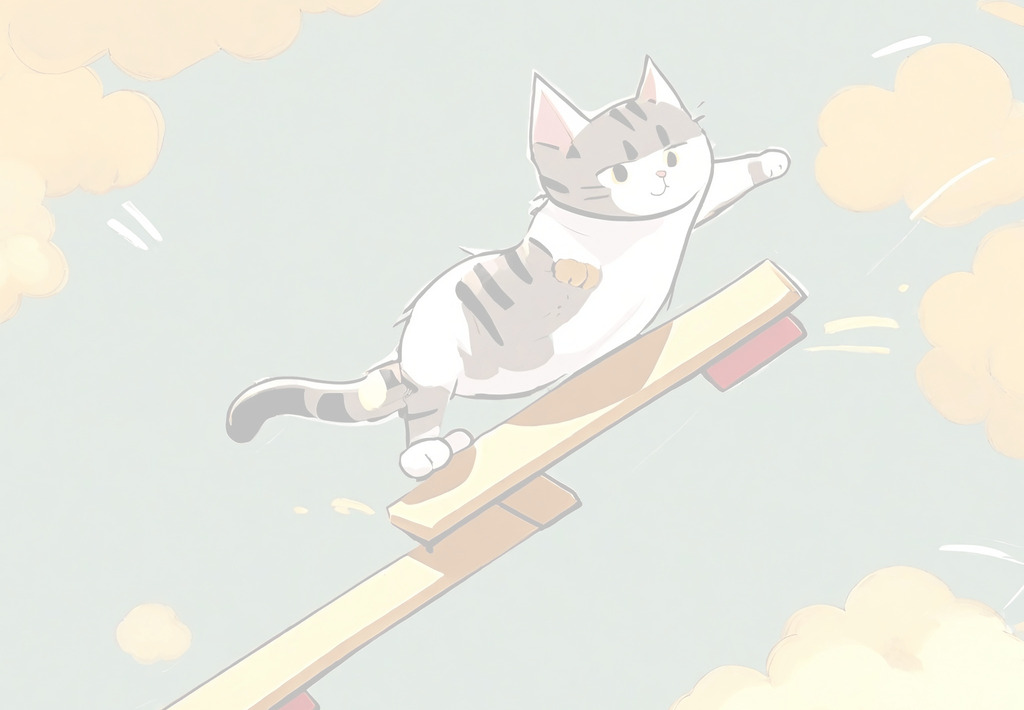
\includegraphics[scale=4.2]{./res/jpegs/cat-in-sky-fs8.jpeg}}} % Image background
\vspace*{15pt}
{\linespread{1.5}\fontsize{18}{18}\selectfont
\par
可正当它哈哈笑的时候,\par
它也飞起来了!\par
这是怎么回事?\par
刚才不是还坐在翘翘板上吗?\par
怎么现在到了半空啦?\par
\par
\par}
\ClearShipoutPicture


\newpage
\AddToShipoutPicture*{\put(-0,-0){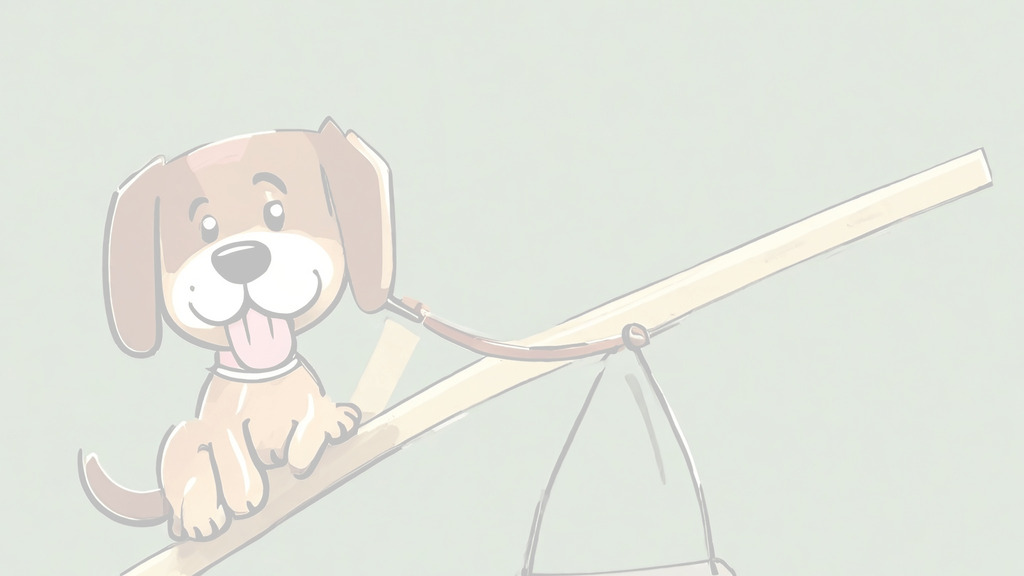
\includegraphics[scale=4.9]{./res/jpegs/dog-on-seesaw-fs8.jpeg}}} % Image background
\vspace*{15pt}
{\linespread{1.5}\fontsize{18}{18}\selectfont
\par
它低头一看,\par
原来是小狗跳到翘翘板上,\par
自己这一边突然被撬起来了!\par
小狗很得意。\par
小猫,你太小了。\par
我一坐下来,\par
你就飞到天上去了!\par
\par
\par}
\ClearShipoutPicture



\newpage
\AddToShipoutPicture*{\put(-0,-0){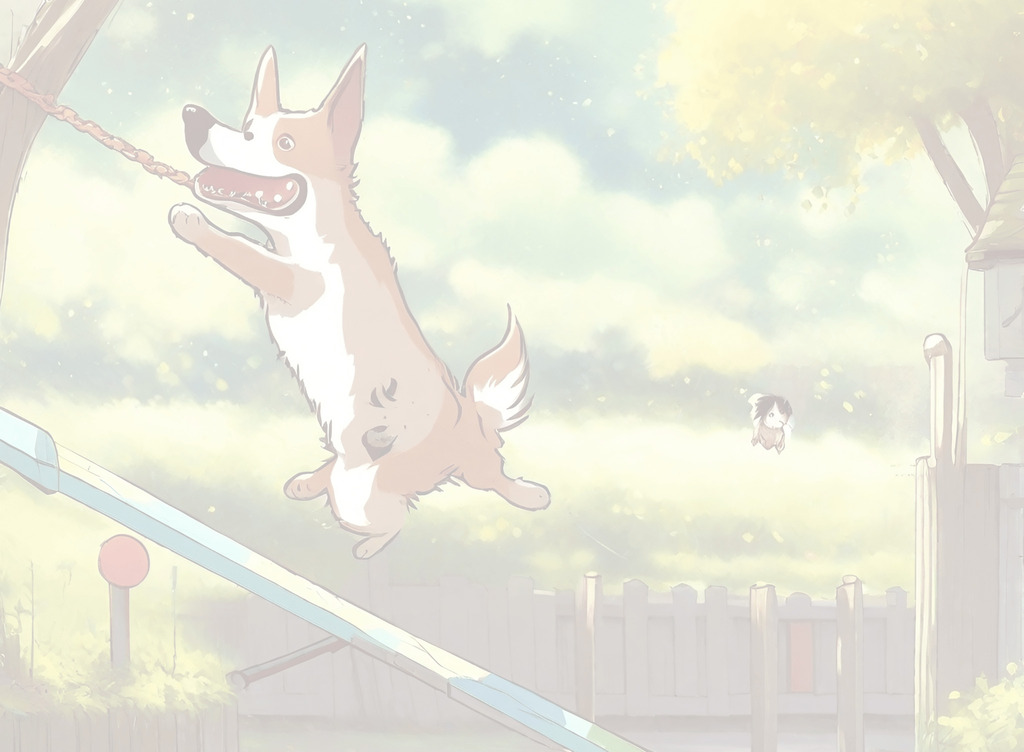
\includegraphics[scale=4.2]{./res/jpegs/dog-in-sky-fs8.jpeg}}} % Image background
\vspace*{15pt}
{\linespread{1.5}\fontsize{18}{18}\selectfont
\par
可正当它哈哈笑的时候,\par
它也飞起来了!\par
这是怎么回事?\par
刚才不是还坐在翘翘板上吗?\par
怎么现在到了半空啦?\par
\par
\par}
\ClearShipoutPicture



\newpage
\AddToShipoutPicture*{\put(-50,-80){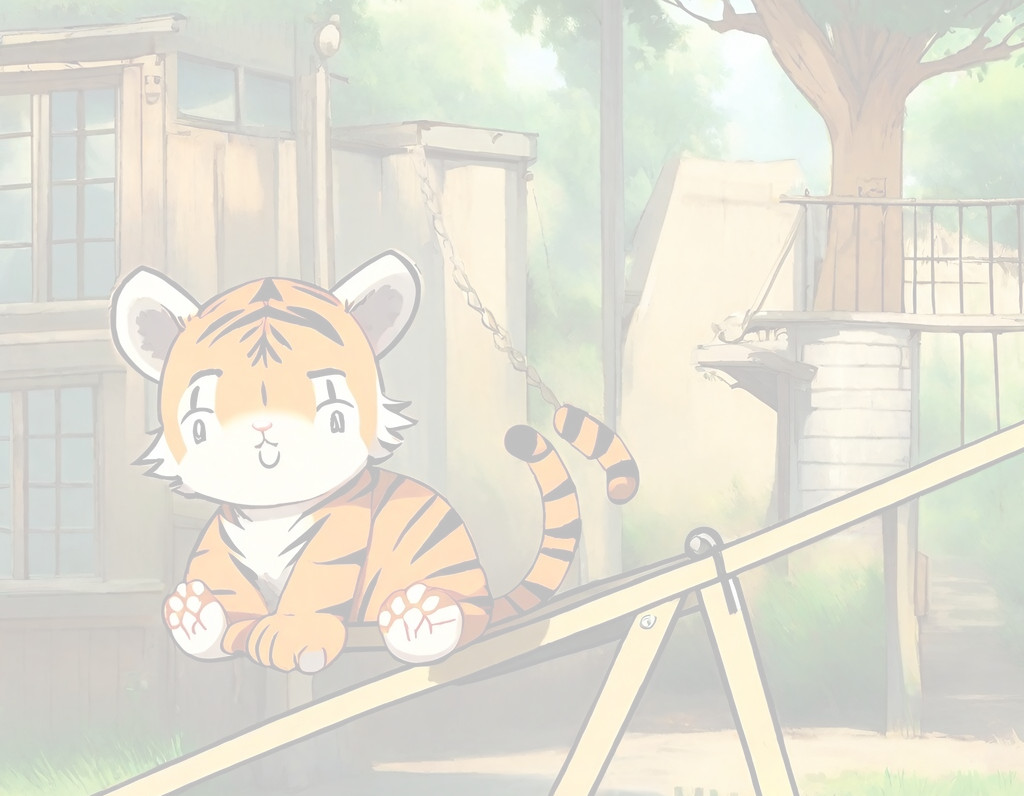
\includegraphics[scale=1.2]{./res/jpegs/tiger-on-seesaw.jpeg}}} % Image background
\vspace*{15pt}
{\linespread{1.5}\fontsize{18}{18}\selectfont
\par
它低头一看,\par
原来是小老虎跳到翘翘板上,\par
自己这一边突然被撬起来了!\par
小虎很得意。\par
小狗,你太小了。\par
我一坐下来,\par
你就飞到天上去了!\par
\par
\par}
\ClearShipoutPicture



\newpage
\AddToShipoutPicture*{\put(-50,-80){
\includegraphics[scale=1.2]{./res/jpegs/tiger-in-sky.jpeg}}} % Image background
\vspace*{15pt}
{\linespread{1.5}\fontsize{18}{18}\selectfont
\par
可正当它哈哈笑的时候,\par
它也飞起来了!\par
这是怎么回事?\par
刚才不是还坐在翘翘板上吗?\par
怎么现在到了半空啦?\par
\par

\par}
\ClearShipoutPicture



\newpage
\AddToShipoutPicture*{\put(-50,-80){
\includegraphics[scale=4.2]{./res/jpegs/elephant-on-seesaw-fs8.jpeg}}} % Image background
\vspace*{15pt}
{\linespread{1.5}\fontsize{18}{18}\selectfont
\par
它低头一看,\par
原来是大象跳到翘翘板上,\par
自己这一边突然被撬起来了!\par
大象很得意。\par
小老虎,你太小了。\par
我一坐下来,\par
你就飞到天上去了!\par
\par
\par}
% \ClearShipoutPicture



\newpage
\AddToShipoutPicture*{\put(-5,-8){
\includegraphics[scale=1.2]{./res/jpegs/elephant_huge.jpeg}}} % Image background
\vspace*{15pt}
{\linespread{1.5}\fontsize{18}{18}\selectfont
\par
大象哈哈笑着说,\par
我是陆地上最大的动物,\par
你们所有人都撬不动我!\par
\par
\par}
\ClearShipoutPicture



\newpage
\AddToShipoutPicture*{\put(-50,-80){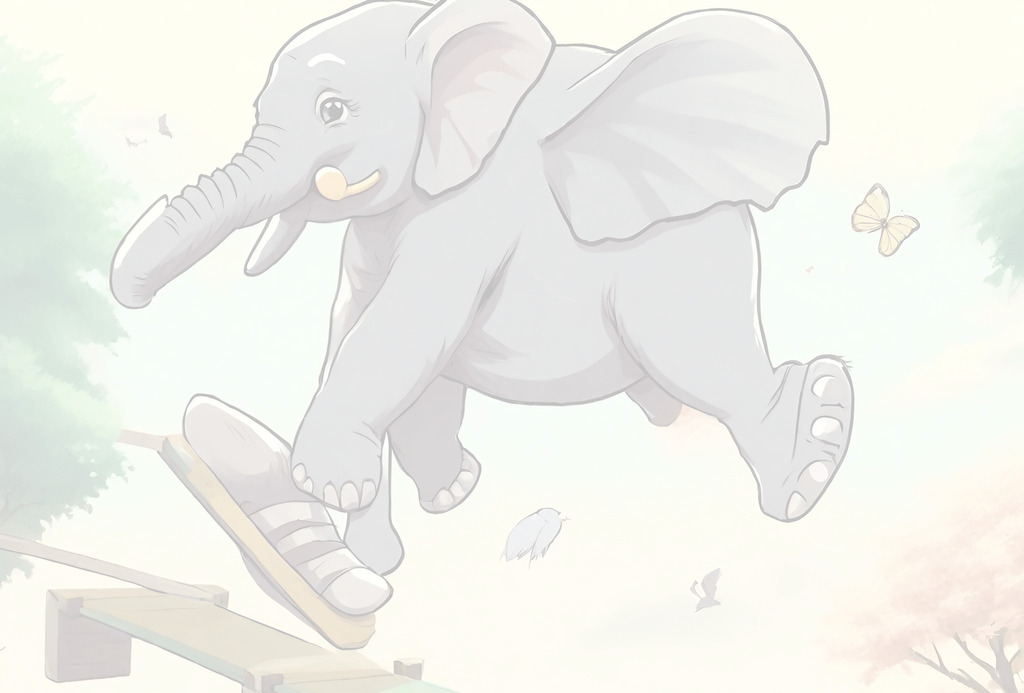
\includegraphics[scale=4.2]{./res/jpegs/elephant-in-sky-fs8.jpeg}}} % Image background
\vspace*{15pt}
{\linespread{1.5}\fontsize{18}{18}\selectfont
\par
\par
可正当它哈哈笑的时候,\par
它也飞起来了!\par
这怎么可能?\par
\par
\par}
\ClearShipoutPicture

\newpage
\AddToShipoutPicture*{\put(-150,-8){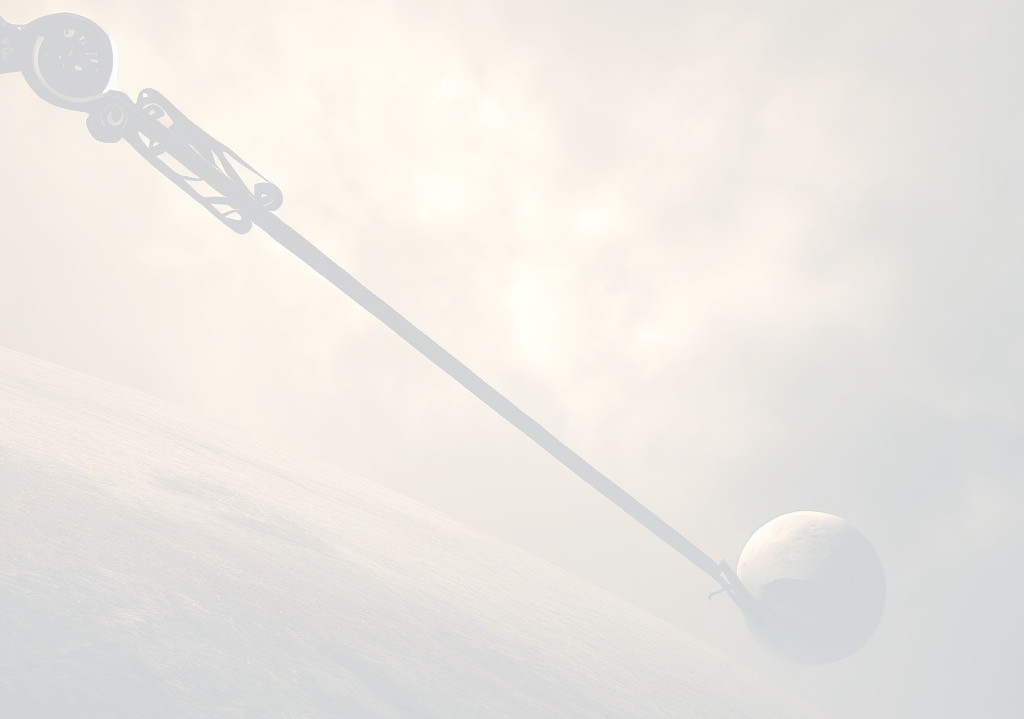
\includegraphics[scale=1.5]{./res/jpegs/earth-leverage.jpeg}}} % Image background
\vspace*{15pt}
{\linespread{1.5}\fontsize{18}{18}\selectfont
\par
\par
它低头一看,\par
原来是小动物们把翘翘板的另一边加长啦,\par
翘翘板变成了大杠杆,\par
自己这一边突然被撬起来了!\par
\par
\par}
\ClearShipoutPicture






\pagenumbering{gobble}
\newpage
\thispagestyle{empty}
\EANisbn[ISBN=978-80-7340-097-2]
\end{multicols}

\end{document}
